\documentclass[english,letter paper,12pt,leqno]{article}
\usepackage{stmaryrd}
\usepackage{amsmath, amscd, amssymb, mathrsfs, accents, amsfonts,amsthm}
\usepackage[all]{xy}
\usepackage{dsfont}
\usepackage{tikz}
\def\nicedashedcolourscheme{\shadedraw[top color=blue!22, bottom color=blue!22, draw=gray, dashed]}
\def\nicecolourscheme{\shadedraw[top color=blue!22, bottom color=blue!22, draw=white]}
\def\nicepalecolourscheme{\shadedraw[top color=blue!12, bottom color=blue!12, draw=white]}
\def\nicenocolourscheme{\shadedraw[top color=gray!2, bottom color=gray!25, draw=white]}
\def\nicereallynocolourscheme{\shadedraw[top color=white!2, bottom color=white!25, draw=white]}
\definecolor{Myblue}{rgb}{0,0,0.6}
\usepackage[a4paper,colorlinks,citecolor=Myblue,linkcolor=Myblue,urlcolor=Myblue,pdfpagemode=None]{hyperref}

\SelectTips{cm}{}

\setlength{\evensidemargin}{0.1in}
\setlength{\oddsidemargin}{0.1in}
\setlength{\textwidth}{6.3in}
\setlength{\topmargin}{0.0in}
\setlength{\textheight}{8.5in}
\setlength{\headheight}{0in}

\newtheorem{theorem}{Theorem}[section]
\newtheorem{proposition}[theorem]{Proposition}
\newtheorem{lemma}[theorem]{Lemma}
\newtheorem{corollary}[theorem]{Corollary}
\newtheorem{setup}[theorem]{Setup}

\newtheoremstyle{example}{\topsep}{\topsep}
	{}
	{}
	{\bfseries}
	{.}
	{2pt}
	{\thmname{#1}\thmnumber{ #2}\thmnote{ #3}}
	
	\theoremstyle{example}
	\newtheorem{definition}[theorem]{Definition}
	\newtheorem{example}[theorem]{Example}
	\newtheorem{remark}[theorem]{Remark}
	\newtheorem{strat}[theorem]{Strategy}

\numberwithin{equation}{section}

% Operators
\def\eval{\operatorname{ev}}
\def\res{\operatorname{Res}}
\def\Coker{\operatorname{Coker}}
\def\Ker{\operatorname{Ker}}
\def\im{\operatorname{Im}}
\def\can{\operatorname{can}}
\def\K{\mathbf{K}}
\def\D{\mathbf{D}}
\def\N{\mathbf{N}}
\def\LG{\mathcal{LG}}
\def\Ab{\operatorname{Ab}}
\def\stab{\operatorname{stab}}
\def\Hom{\operatorname{Hom}}
\def\modd{\operatorname{mod}}
\def\Modd{\operatorname{Mod}}
\def\be{\begin{equation}}
\def\ee{\end{equation}}
\def\nN{\mathds{N}}
\def\nZ{\mathds{Z}}
\def\nQ{\mathds{Q}}
\def\nR{\mathds{R}}
\def\nC{\mathds{C}}
\DeclareMathOperator{\Ext}{Ext}
\DeclareMathOperator{\Tr}{Tr}
\DeclareMathOperator{\End}{End}
\DeclareMathOperator{\rank}{rank}
\DeclareMathOperator{\tot}{Tot}
\DeclareMathOperator{\ch}{ch}
\DeclareMathOperator{\str}{str}
\DeclareMathOperator{\hmf}{hmf}
\DeclareMathOperator{\HMF}{HMF}
\DeclareMathOperator{\hf}{HF}
\DeclareMathOperator{\At}{At}
\DeclareMathOperator{\Cat}{Cat}
\DeclareMathOperator{\Spec}{Spec}

\begin{document}

% Commands
\def\Res{\res\!}
\newcommand{\ud}{\mathrm{d}}
\newcommand{\Ress}[1]{\res_{#1}\!}
\newcommand{\cat}[1]{\mathcal{#1}}
\newcommand{\lto}{\longrightarrow}
\newcommand{\xlto}[1]{\stackrel{#1}\lto}
\newcommand{\mf}[1]{\mathfrak{#1}}
\newcommand{\md}[1]{\mathscr{#1}}
\def\sus{\l}
\def\l{\,|\,}
\def\sgn{\textup{sgn}}

\title{$A_\infty$-minimal models of matrix factorisations}
\author{Daniel Murfet}

\maketitle

\begin{abstract}
We study $A_\infty$-minimal models of the differential graded algebras obtained from endomorphisms of generators of triangulated categories of matrix factorisations, giving explicit higher products for the cases of simple singularities. 
\end{abstract}

\section{Introduction}

Let $k$ be a commutative $\mathbb{Q}$-algebra and $W \in k[x_1,\ldots,x_n]$ a polynomial which is a potential over $k$ in the sense of \cite[\S 2.2]{lgdual}. For example, $k = \mathbb{C}$ and $W$ has isolated critical points. The $\nZ_2$-graded DG-category $\cat{A} = \operatorname{mf}(R, W)$ has for its objects finite-rank matrix factorisations of $W$ over $R = k[x_1,\ldots,x_n]$. In this paper we study the minimal model problem for $\cat{A}$, the aim being to produce models that are finitely-generated and projective over $k$.

When $k$ is a field, the standard minimal model theorem \cite{??} constructs the structure of an $A_\infty$-category on the cohomology $\cat{B} = H^* \cat{A}$ in such a way that $\cat{B}$ is quasi-isomorphic to $\cat{A}$. Moreover, this $A_\infty$-category has finite-dimensional Hom-spaces and is therefore a good finite model of $\cat{A}$. The problem in this case is to have sufficient control over the inputs to the minimal model theorem that the $A_\infty$-products on $H^* \cat{A}(X,X)$ can be reasonably calculated, for a given matrix factorisation $X$. In order to understand deformations of matrix factorisations \cite{??,??,??} it is important to do this for generic $X$, but the special case where $X = k^{\stab}$, the generator of $\cat{A}$ studied by Dyckerhoff in the case of a single isolated singularity at the origin \cite{d0904.4713}, is of particular interest.

Since one of our goals is to understand how matrix factorisation categories vary along unfoldings of singularities, we also need to consider the case where $k$ is not a field. For example take $k = \mathbb{C}[t]$ and $R = \mathbb{C}[x_1,\ldots,x_n, t]$ so that $W = W_t(x)$ is a potential with parameter. In this case we want an $A_\infty$-category $\cat{B}$ quasi-isomorphic to $\cat{A}$ over $k$, with $\cat{B}(a,b)$ a finitely-generated projective $k$-module for each pair of objects $a,b$. 
\vspace{0.2cm}

These two desiderata, understanding the $A_\infty$-products on $H^*\cat{A}(X,X)$ for generic $X$, and the case where $k$ is not a field, lead us naturally to a slightly non-standard use of the minimal model theorem. Following the ideas developed in \cite{??,??,??} we prove that, writing $\iota: R \lto R/(\partial_{x_1} W, \ldots, \partial_{x_n} W)$ for the quotient, there is a $k$-linear homotopy retract
\be\label{eq:intro_he}
\xymatrix@C+4pc{
\iota^* \cat{A} \ar@<0.7ex>[r] & \cat{A} \otimes_k \bigwedge\big( k^{\oplus n}[1] \big) \ar@<0.7ex>[l]\,.
}
\ee

Suppose $W \in \mf{m}^2$ where $\mf{m} = (x_1,\ldots,x_n)$ and choose a presentation $W = x_1 W^1 + \cdots + x_n W^n$ with $W^i \in \mf{m}$ and consider the following pair
\begin{equation}\label{eq:kstab}
k^{\operatorname{stab}} = \Big( k[x] \otimes_k \bigwedge( k\psi_1 \oplus \cdots \oplus k \psi_n ), \;d_{k^{\stab}} = \sum_{i=1}^n x_i \psi_i^* + \sum_{i=1}^n W^i \psi_i \Big)
\end{equation}
where $\psi_i^*$ and $\psi_i$ act respectively by contraction and wedge product on the exterior algebra underlying $k^{\stab}$. It is easy to see that $d_{k^{\stab}}^2 = W$, so $k^{\stab}$ is a matrix factorisation. When $k$ is a field and $W$ has an isolated critical point at the origin, $k^{\stab}$ is the representative in the homotopy category of matrix factorisations of the structure sheaf of the singular point at the origin, and was first studied by Dyckerhoff \cite{d0904.4713}. 

The purpose of this paper is to show how to calculate the $A_\infty$-minimal model of the $\nZ_2$-graded differential graded endomorphism algebra of this matrix factorisation
\be\label{eq:defnaw}
\Big( \End_{k[x]}(k^{\operatorname{stab}}), \; \partial = [d_{k^{\stab}},-] \; \Big)\,.
\ee 
The differential here is (throughout all commutators are graded commutators)
\begin{align*}
\partial = [d_{k^{\stab}},-] &= \Big[\sum_i x_i \psi_i^* + \sum_i W^i \psi_i, -\Big]\\
&= \sum_i x_i [\psi_i^*,-] + \sum_i W^i [\psi_i,-]\,.
\end{align*}
The minimal model is a finite-dimensional $\nZ_2$-graded vector space $\md{M}_W$ with a family 
\[
\left\{ r_q: \big(\md{M}_W[1]\big)^{\otimes q} \lto \md{M}_W[1] \right\}_{q \ge 2}
\]
of odd $k$-linear maps satisfying the forward suspended $A_\infty$-constraints \cite{lazaroiu}, and having the property that there is an $A_\infty$-quasi-isomorphism $\md{M}_W \lto \End_{k[x]}(k^{\stab})$.

\section{Background}

\subsection{A-infinity algebras}

The \emph{tilde grading} is defined by $\widetilde{x} = |x| - 1$.

Throughout $\otimes = \otimes_k$.

\section{Perturbation and Koszul complexes}

Let $k$ be a characteristic zero field, $R =  k[x_1,\ldots,x_n]$ and let $W \in \mf{m}^2$ be a potential with chosen decomposition $W = \sum_{i=1}^n x_i W^i$. To apply the $A_\infty$-minimal model construction to the DG-algebra $\md{A}_W$ from \eqref{eq:defnaw} we would usually begin by finding a $k$-linear homotopy retract of this complex onto its cohomology. However, for our purposes it is better to first enlarge the DG-algebra to $S \otimes \md{A}_W$, where $S$ is the $\nZ_2$-graded vector space
\be
S = \bigwedge( k\theta_1 \oplus \cdots \oplus k \theta_n )
\ee
with grading $|\theta_i| = 1$. We make the tensor product $S \otimes \md{A}_W$ into a DG-algebra in the usual way, giving the exterior algebra $S$ the zero differential.

\begin{definition} We define the finite-dimensional $\nZ_2$-graded vector space
\be\label{eq:defnunderlineend}
\md{E} = R/\mf{m} \otimes \End_R(k^{\stab}) \cong \End_k\Big( \bigwedge( k\psi_1 \oplus \cdots \oplus k \psi_n) \Big)
\ee
where $\mf{m} = (x_1,\ldots,x_n)$.
\end{definition}

We will show that $S \otimes \md{A}_W$ is homotopy equivalent to $\md{E}$ viewed as a complex with zero differential (observe that $\md{E}$ does not depend on $W$). The corresponding homotopy retract (see Proposition \ref{prop:he_start} below) is our starting point for the minimal model construction. For this we use the Koszul complex of $x_1,\ldots,x_n$,
\be\label{eq:defnkoszulK}
K = \Big( R \otimes \bigwedge( k\theta_1 \oplus \cdots \oplus k \theta_n ), \; d_K = \sum_i x_i \theta_i^*\; \Big)
\ee

\begin{theorem} There is a diagram of $\nZ_2$-graded complexes and homotopy equivalences over $k$
\be\label{eq:first_he}
\xymatrix@C+3pc{
S \otimes \md{A}_W \ar@<1ex>[r]^-{\exp(-\delta)} & K \otimes_R \md{A}_W \ar@<1ex>[l]^-{ \exp(-\delta) } \ar@<1ex>[r]^-{\pi} & \md{E}\,.\ar@<1ex>[l]^-{ \sigma_\infty }
}
\ee
\end{theorem}
\begin{proof}
See \cite{murfet}.
\end{proof}

The notation is as follows:
\begin{itemize}
\item The complexes involved here are
\begin{gather*}
\big( S \otimes \End_R(k^{\stab}), \; \partial \,\big)\\
\big( K \otimes_R \End_R(k^{\stab}), \; d_K + \partial\, \big)\\
\big( \md{E}, 0 \big)\,.
\end{gather*}
\item The operator $\psi_j = \psi_j \wedge -$ on $k^{\stab}$ satisfies
\[
[ \psi_j, d_{k^{\stab}} ] = \big[ \psi_j, \sum_i x_i \psi_i^* \big] = x_j \cdot 1\,,
\]
where $[-,-]$ always denotes the graded commutator. That is, $\psi_j$ is a homotopy for the action of $x_j$ on $k^{\stab}$. It is then easy to check that the odd operator $\alpha \mapsto \psi_j \circ \alpha$ on $\End_R(k^{\stab})$ is also a homotopy for $x_j$, and where it will not cause confusion we will also write $\psi_j$ for this operator of post-composition.

\item Both $S \otimes \md{A}_W$ and $K \otimes_R \md{A}_W$ have the same underlying $\nZ_2$-graded $k$-module, namely
\be\label{eq:same_underlying}
R \otimes \bigwedge( k\theta_1 \oplus \cdots \oplus k \theta_n ) \otimes \End_k\big( \bigwedge( k\psi_1 \oplus \cdots \oplus k \psi_n ) \big)\,.
\ee
On this space we define the even operator
\be
\delta = \sum_{i=1}^n \psi_i \theta_i^*\,,
\ee
where $\psi_i$ is the operator on $\End_R(k^{\stab})$ discussed above, given by $\alpha \mapsto (\psi_i \wedge -) \circ \alpha$, and $\theta_i^*$ acts by contraction on $S$. It is easy to check that $\exp(\delta),\exp(-\delta)$ intertwines the differentials $\partial$ and $d_K + \partial$ and therefore gives an isomorphism between the first two complexes in \eqref{eq:first_he} \cite[Proposition 4.11]{murfet}.
\item The morphism of complexes $\pi: K \lto R/\mf{m}$ is defined by composing the projection of $K$ onto the submodule $R \cdot 1$ of $\theta$-degree zero forms, with the quotient $R \lto R/\mf{m}$. We also write $\pi$ for the result of tensoring this morphism with $\End_R(k^{\stab})$ to obtain
\[
\xymatrix@C+2pc{
K \otimes_R \End_R(k^{\stab}) \ar[r]^-{\pi \otimes 1} & R/\mf{m} \otimes_R \End_R(k^{\stab}) = \underline{\End}(k^{\stab})\,.
}
\]
This is a morphism of complexes, because the differential on $\End_R(k^{\stab})$ vanishes on the quotient $\underline{\End}(k^{\stab})$ by the hypothesis that $W \in \mf{m}^2$.
\item The $k$-linear homotopy inverse $\sigma_\infty$ to $\pi$ in \eqref{eq:first_he} is defined in terms of the following ingredients. The first is the $k$-linear connection (viewing $\theta_i$ as a $1$-form)
\be
\Delta: K \lto K\,, \qquad \Delta = \sum_i \partial_{x_i} \theta_i
\ee
and the degree $-1$ (with respect to the $\theta$-degree) $k$-linear operator
\be
H = [d_K, \Delta]^{-1} \Delta\,.
\ee
We write $\partial$ for the differential on $\End_R(k^{\stab})$, and $\sigma: k \lto K$ for the map which sends $\lambda \in k$ to $\lambda \cdot 1 \in K$, and define $k$-linear maps
\begin{align}
\sigma_\infty = \sum_{m \ge 0} (-1)^m (H \partial)^m \sigma\,,\\
H_\infty = \sum_{m \ge 0} (-1)^m (H \partial)^m H\,.
\end{align}
Here $H_\infty$ is an odd operator on $K \otimes_R \End_R(k^{\stab})$. These maps satisfy:
\begin{align}
\pi \sigma_\infty &= 1\,,\\
 \sigma_\infty \pi &= 1 - [d_K + \partial, H_\infty]\,.
\end{align}
\end{itemize}

By inspection of \eqref{eq:first_he}, we therefore have the following:

\begin{proposition}\label{prop:he_start} There is a diagram of morphisms of $\nZ_2$-graded $k$-complexes
\be\label{eq:he_start}
\xymatrix@C+5pc{
S \otimes \md{A}_W \ar@<1ex>[r]^-{\Phi} & \md{E}\ar@<1ex>[l]^-{\Phi^{-1}}
}
\ee
where $\Phi = \pi \exp(-\delta), \Phi^{-1} = \exp(\delta) \sigma_\infty$ and $\widehat{H} = \exp(\delta) H_\infty \exp(-\delta)$ satisfy
\be
\Phi \Phi^{-1} = 1\,, \qquad \Phi^{-1} \Phi = 1 - [\partial, \widehat{H}]\,.
\ee
Thus, $\Phi$ and $\Phi^{-1}$ are mutually inverse homotopy equivalences over $k$.
\end{proposition}

The endomorphism algebra $C = \End_k(S)$ is a Clifford algebra generated by the contraction $\theta_i^*$ and wedge product $\theta_i$ operators. It is observed in \cite{murfet} that \eqref{eq:he_start} is an isomorphism of Clifford representations (in the homotopy category) when the complex $\md{E}$ is equipped with the action induced by Atiyah classes:

\begin{definition}
The Atiyah classes of $\md{A}_W$ are the $R$-linear odd operators
\[
\At_i = [\partial, \partial_{x_i}]: \End_R(k^{\stab}) \lto \End_R(k^{\stab})\,,
\]
\end{definition}

\begin{lemma} We have
\[
\At_i = -[\psi_i^*, -] - \sum_{q=1}^n \partial_{x_i}(W^q) [ \psi_q, - ]\,.
\]
\end{lemma}
\begin{proof}
By direct calculation:
\begin{align*}
\At_i &= \big[ [d_{k^{\stab}},-], \partial_{x_i} \big]\\
&= \sum_q \big[x_q [\psi_q^*,-], \partial_{x_i}\big] + \sum_q \big[W^q [\psi_q,-], \partial_{x_i}\big]\\
&= -\sum_q \partial_{x_i}(x_q) [\psi_q^*,-] - \sum_q \partial_{x_i}(W^q) [\psi_q,-]\\
&= -[\psi_i^*,-] - \sum_q \partial_{x_i}(W^q) [\psi_q, -]\,.
\end{align*}
\end{proof}

\section{The minimal model}

We now take the homotopy retract from Proposition \ref{prop:he_start} as the input to the usual algorithm for the construction of an $A_\infty$-minimal model of the DG-algebra $S \otimes \md{A}_W$. We make use of the forward suspended products for this DG-algebra, which are
\be
r_q: \left( S \otimes \md{A}_W [1] \right)^{\otimes q} \lto S \otimes \md{A}_W[1]
\ee
defined to be zero except for $r_1 = \partial$ and 
\be
r_2( \alpha \otimes \beta ) = (-1)^{\widetilde{\alpha} \widetilde{\beta} + \widetilde{\beta} + 1} \beta \alpha
\ee
where $\beta \alpha$ is the usual product in $S \otimes_ k \md{A}_W$ and $\widetilde{\alpha} = |\alpha| - 1$. Applying the algorithm described in Section \ref{??} to the data of the $A_\infty$-algebra $\big( S \otimes \md{A}_W, \{ r_1, r_2 \} \big)$ and the strong homotopy retract of Proposition \ref{prop:he_start} produces a minimal $A_\infty$-algebra
\[
\big( \md{E}, \{ \rho_q \}_{q \ge 2} \big)\,.
\]
The products are defined by sums over trees, for example: one tree contributing to $\rho_3$ is:
\begin{center}
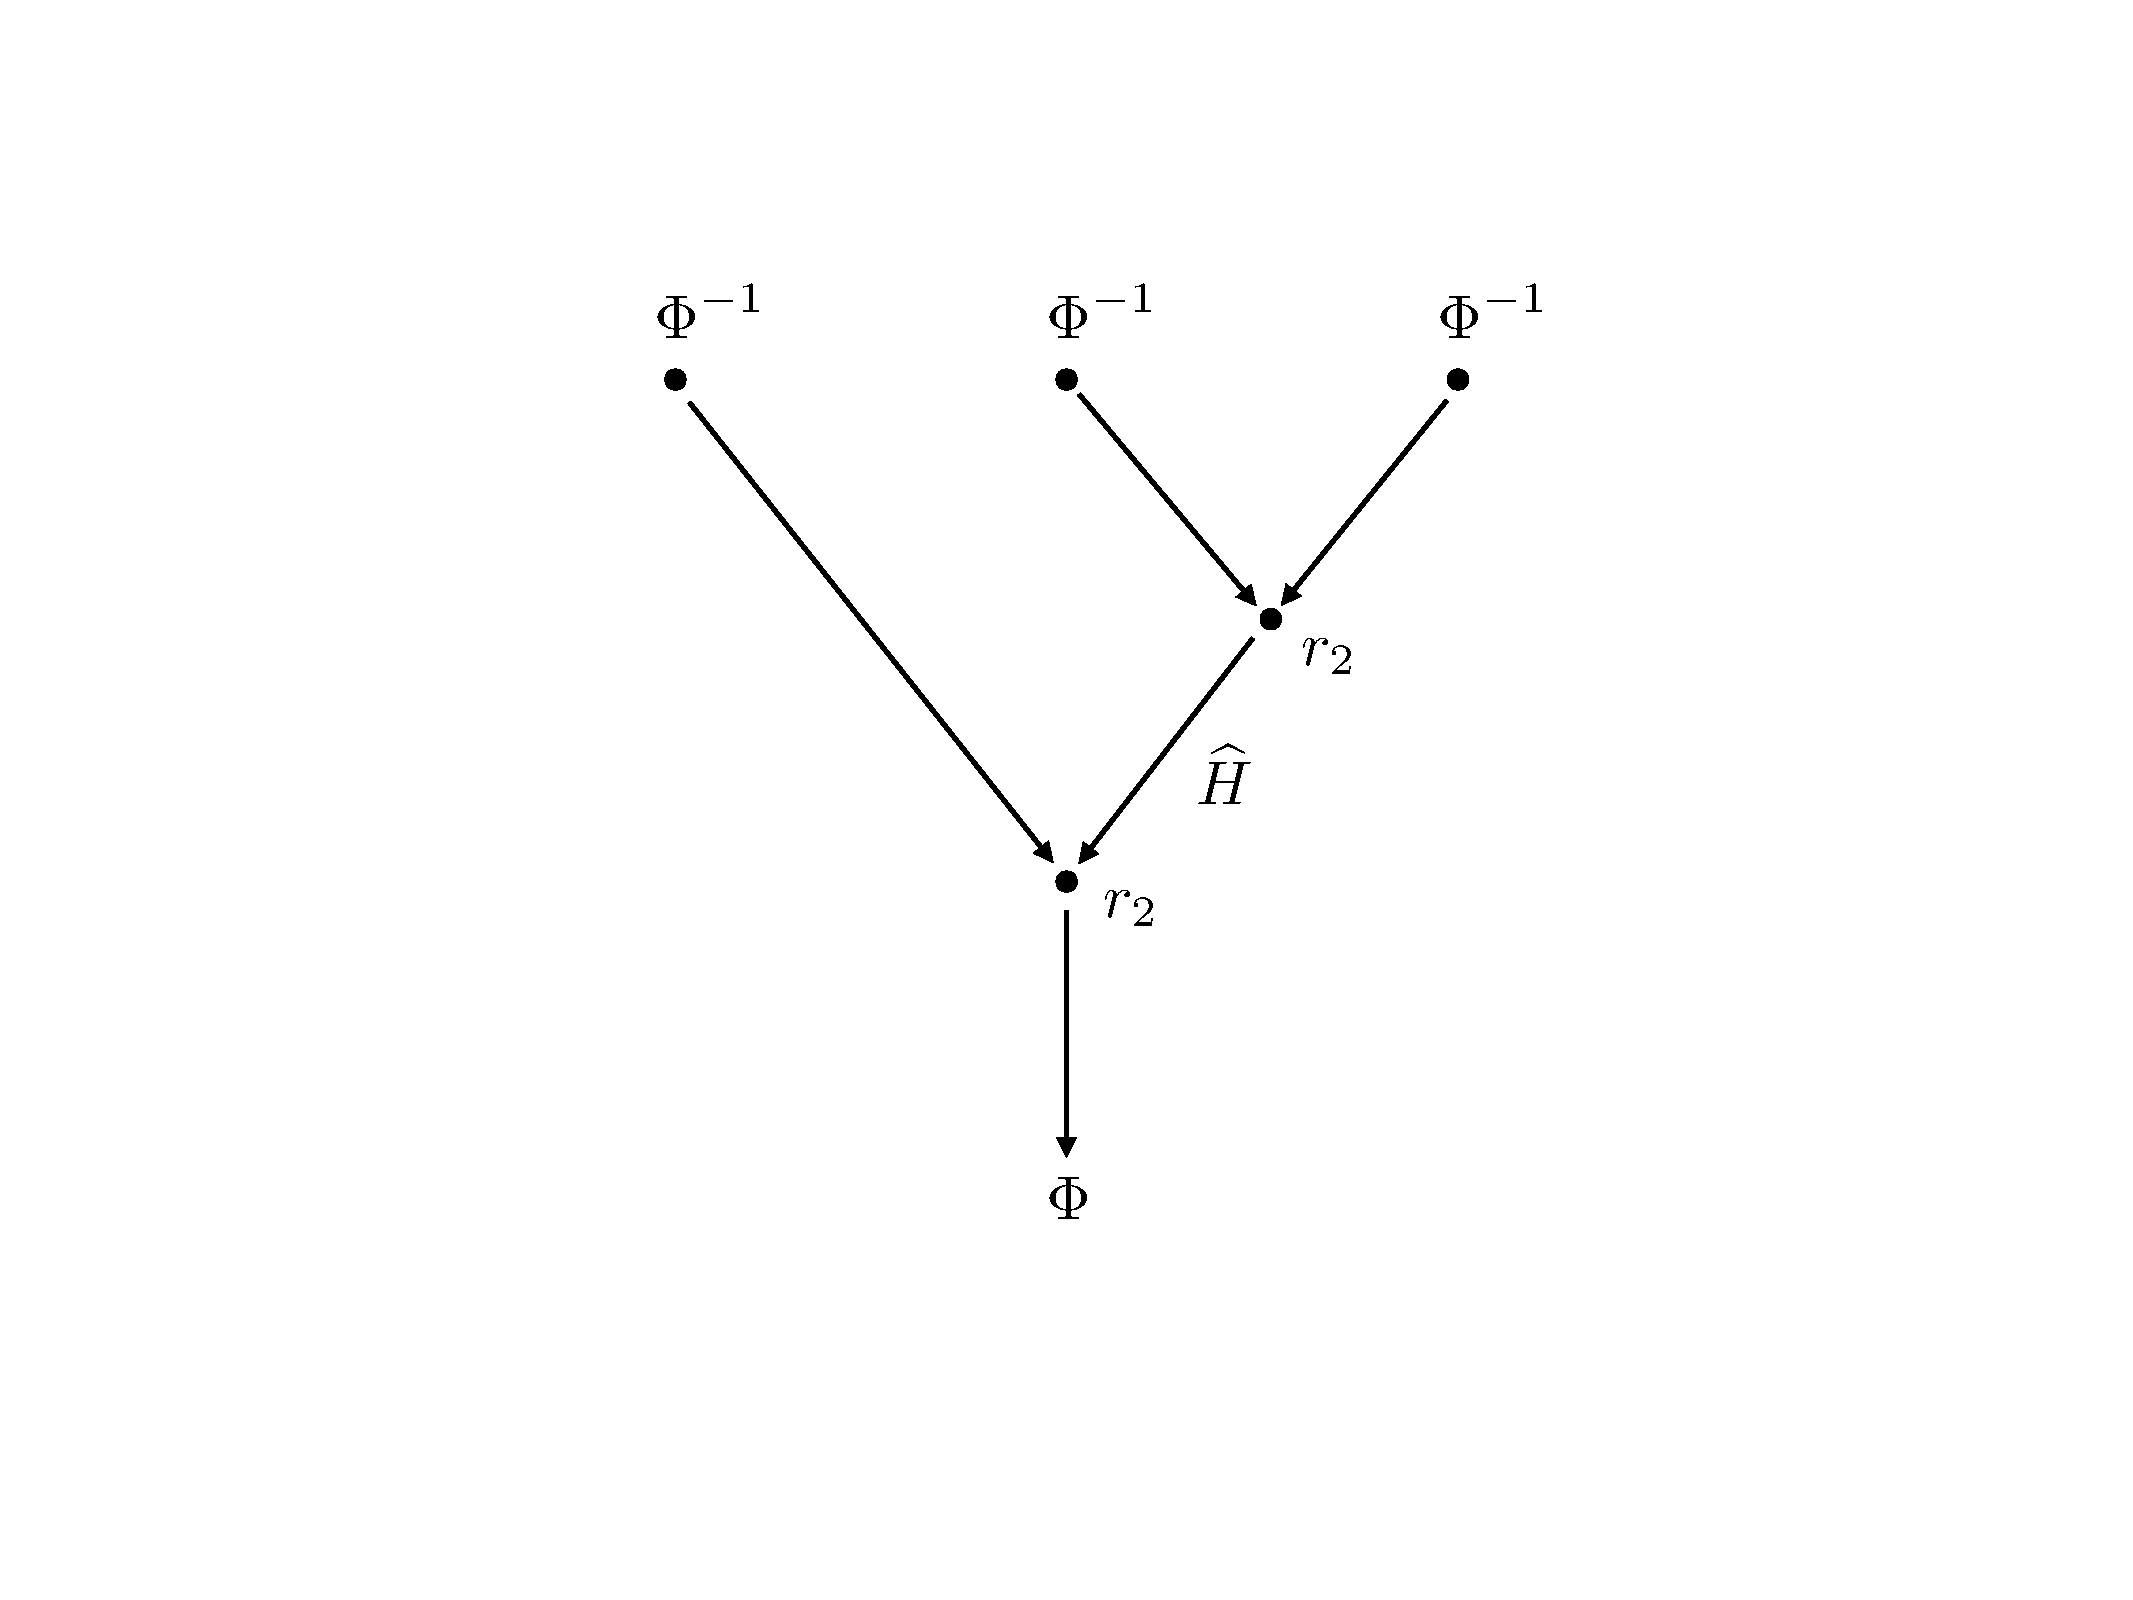
\includegraphics[scale=0.35]{diagram-1}
\end{center}
For this particular tree $T$ the associated operator is
\[
\rho_T = (-1)^1 \Phi \circ r_2 \circ ( \Phi^{-1} \otimes \widehat{H} ) \circ ( 1 \otimes r_2 ) \circ (1 \otimes \Phi^{-1} \otimes \Phi^{-1} ) \,.
\]
We first describe the final algorithm which allows us to compute the operations $\rho_q$ in terms of the Feynman rules, and then we will justify this algorithm in the remainder of the paper. Here we stick to $W \in \mf{m}^3$ and consider the subalgebra of $\md{E}$ generated by the contraction operators
\[
\md{M} = \bigwedge( k\psi_1^* \oplus \cdots \oplus k \psi_n^* ) \subseteq \md{E}\,.
\]
The formula is expressed in terms of \emph{vacuum amplitudes} which are functionals defined for every tree $T$ with $q$ input vertices
\[
\cat{O}(T) \in (\md{M}^{\otimes q})^*
\]
This amplitude is defined to be a sum over \emph{configurations}
\[
\cat{O}(T) = \sum_{c \in \cat{C}} \cat{O}(T, c)\,.
\]
\newpage

We define the even operator $\delta_i = \psi_i \theta_i^*$ on the underlying module $\eqref{eq:same_underlying}$ of $S \otimes \md{A}_W$, so that $\delta = \sum_i \delta_i$. Since $[ \delta_i, \delta_j ] = 0$ for all $i,j$ we have
\be
\exp(\pm \delta) = \exp(\pm \delta_1) \cdots \exp(\pm \delta_n)\,.
\ee

\begin{lemma} For $1 \le i \le n$ there is a commutative diagram
\be
\xymatrix@C+3pc@R+1pc{
(S \otimes \md{A}_W) \otimes (S \otimes \md{A}_W) \ar[d]_-{\delta_i \otimes 1 + 1 \otimes \delta_i + [\psi_i,-] \otimes \theta_i^*} \ar[r]^-{m_2} & S \otimes \md{A}_W \ar[d]^-{\delta_i}\\
(S \otimes \md{A}_W) \otimes (S \otimes \md{A}_W) \ar[r]_-{m_2} & S \otimes \md{A}_W
}
\ee
\end{lemma}

\begin{definition} We define
\be
\Xi_i = [ \psi_i, - ] \otimes \theta_i^* : S \otimes \md{A}_W \lto S \otimes \md{A}_W\,.
\ee
and
\be
\Xi = \sum_i \Xi_i\,.
\ee
\end{definition}

\begin{proposition} There is a commutative diagram
\be
\xymatrix@C+3pc@R+2pc{
(S \otimes \md{A}_W) \otimes (S \otimes \md{A}_W) \ar[d]_-{\exp(-\delta) \otimes \exp(-\delta)} \ar[r]^-{m_2} & S \otimes \md{A}_W \ar[dd]^-{\exp(-\delta)}\\
(S \otimes \md{A}_W) \otimes (S \otimes \md{A}_W) \ar[d]_-{\exp(-\Xi)}\\
(S \otimes \md{A}_W) \otimes (S \otimes \md{A}_W) \ar[r]_-{m_2} & S \otimes \md{A}_W
}
\ee
\end{proposition}

\begin{definition} $\eval_T$ is the operator associated to the tree $T$ with $\sigma_\infty$ on all input vertices, $m_2 \exp(-\Xi)$ on all internal vertices and $H_\infty$ on internal edges.
\end{definition}

\begin{lemma} For any tree $T$
\[
\rho_T( \alpha_1 \otimes \cdots \otimes \alpha_q ) = (-1)^{S(T, \ell)} \eval_{\widehat{T}}( \alpha_q \otimes \cdots \otimes \alpha_1 )
\]
where $\ell = (\widetilde{\alpha}_1,\ldots,\widetilde{\alpha}_q)$.
\end{lemma}


\begin{center}
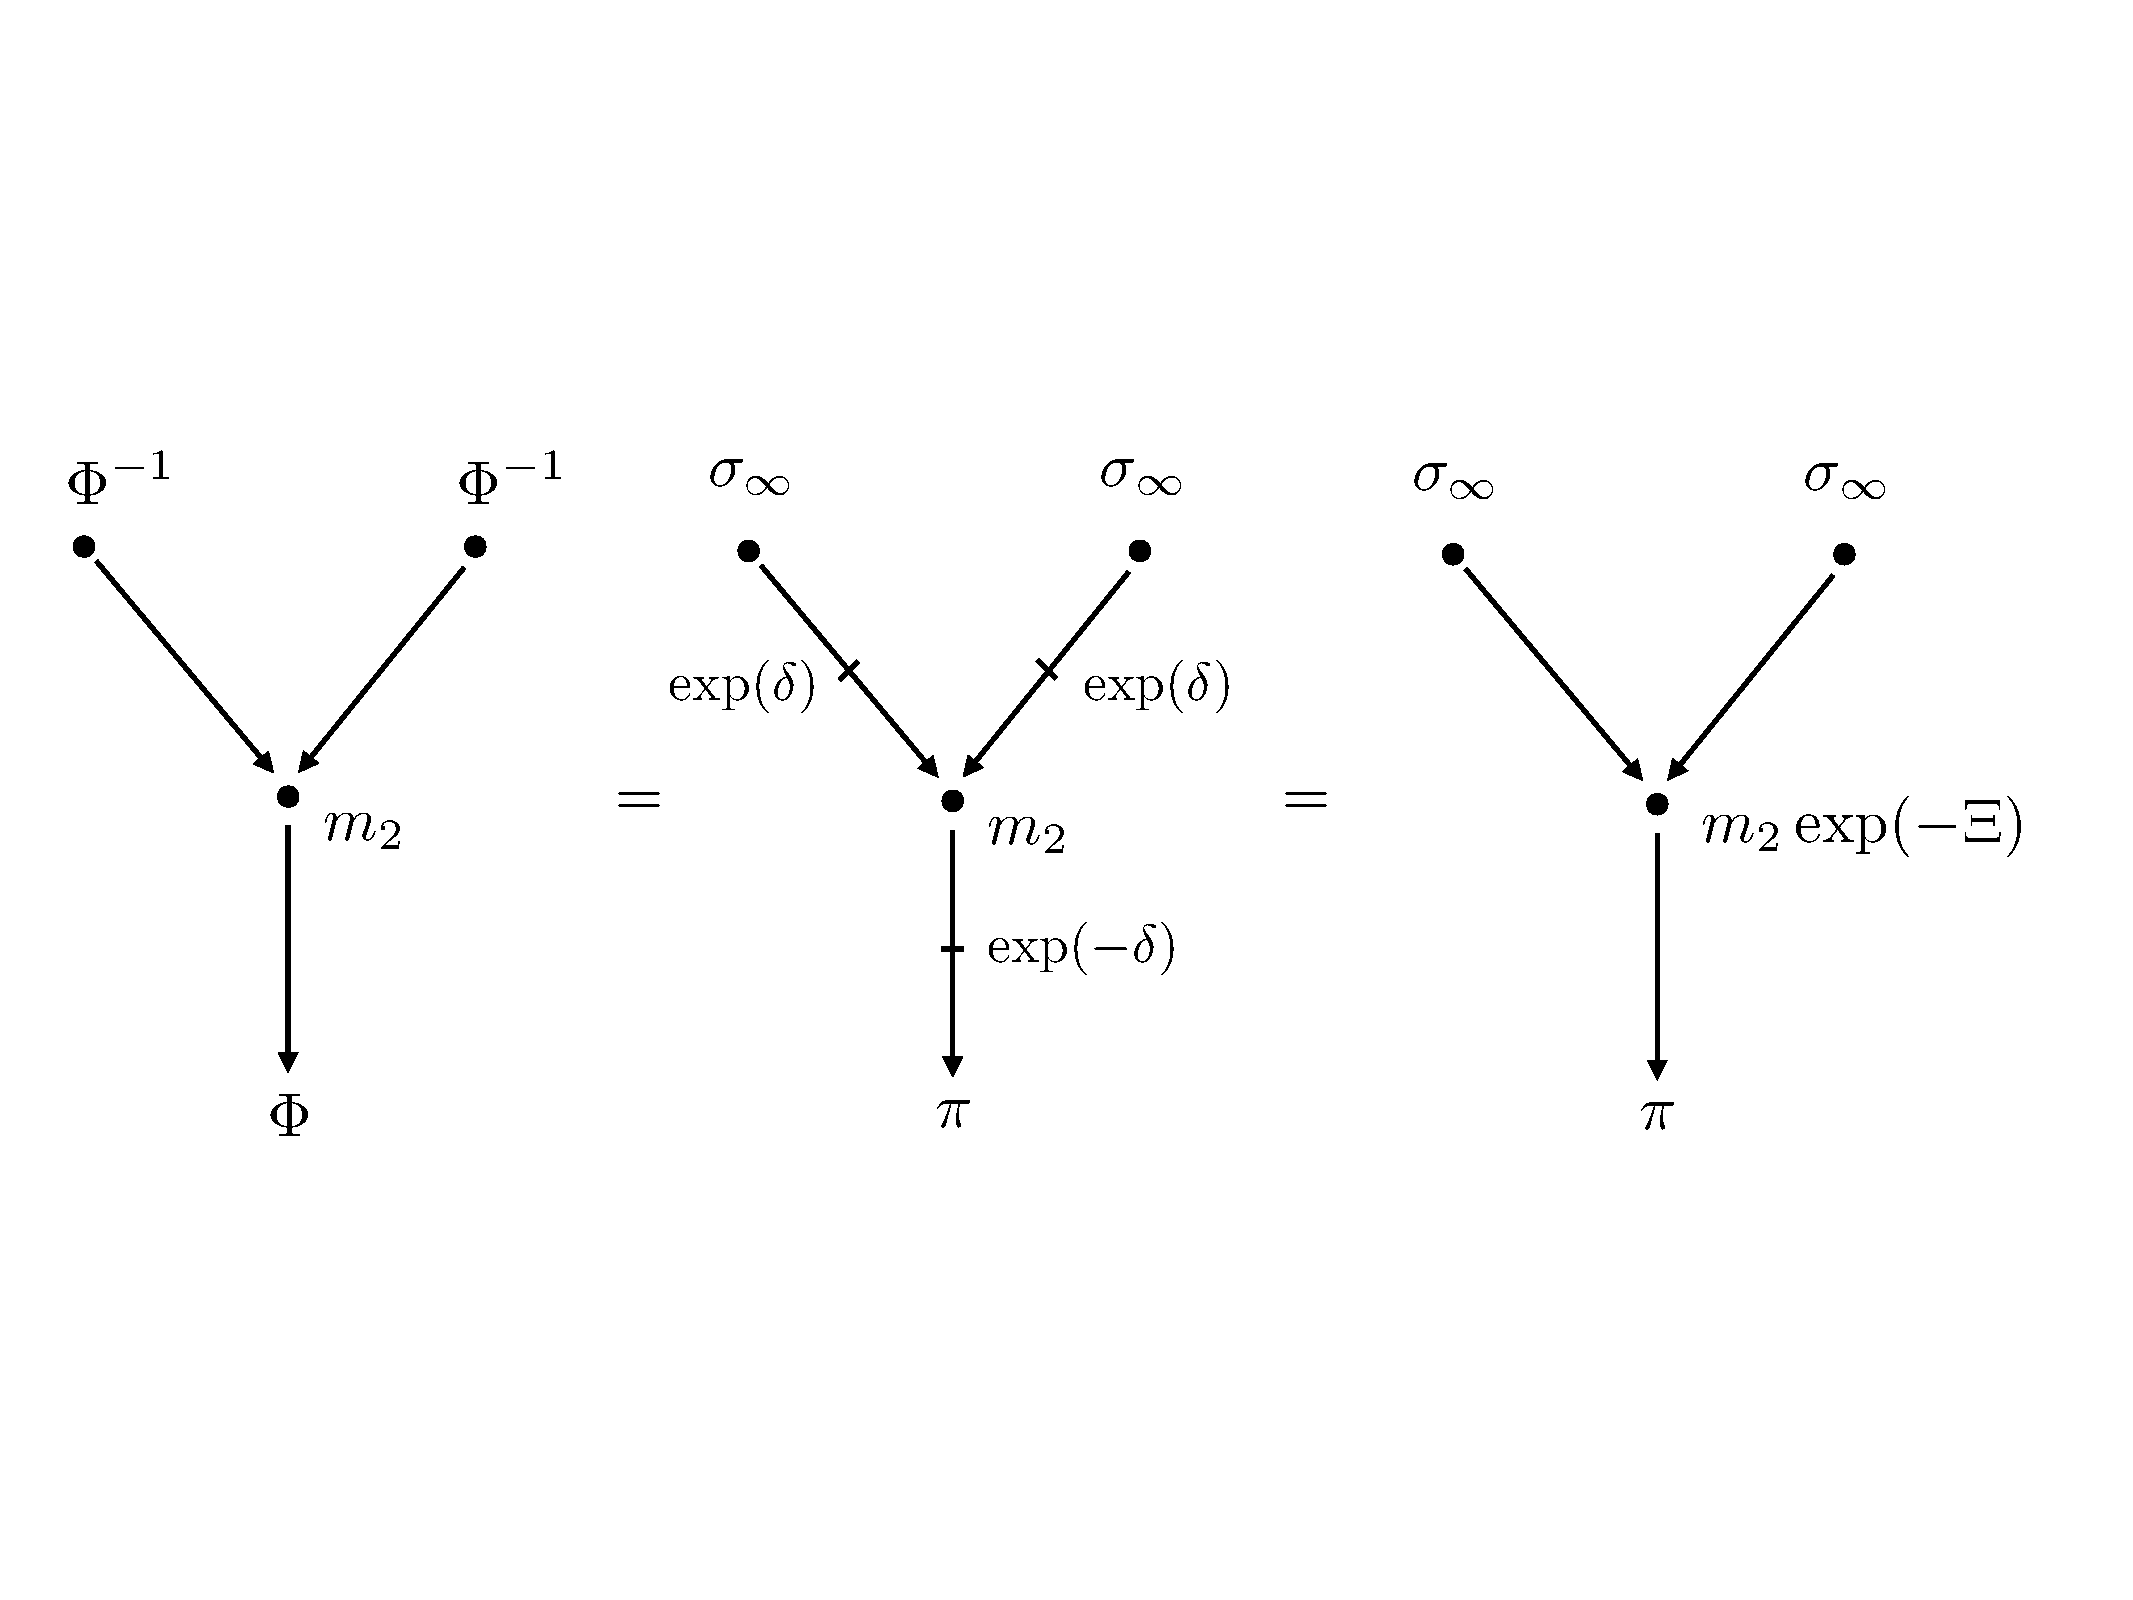
\includegraphics[scale=0.35]{diagram-2}
\end{center}

\section{Notes}

\begin{remark} Varying the potential $W$ affects only the relative ``strength'' of the triple-vertex interactions, which are indexed by the monomials $\gamma$. Thus we can, for example, examine the degeneration from $x^{d+1}$ to $x^d$ (bundles of minimal $A_\infty$-algebras).
\end{remark}

\section{Algorithm}
% from p.17 (ainfmf9)

Let $T \in \cat{T}_q$ be a valid plane tree with $q$ inputs and $e_i(T)$ internal edges, and let $A(T)$ be the augmented plane tree. Recall that the vertices of $A(T)$ may be partitioned into the following subsets: the root, the non-root leaves (called \emph{inputs}), the vertices coming from internal edges of $T$, and those internal vertices coming from internal vertices of $T$. The integer $n$ is the number of variables in the ambient ring $R = k[x_1,\ldots,x_n]$. 

Consider the tensor product
\[
\mathscr{H} = R \otimes_k \bigwedge\big( \oplus_{i=1}^n k \theta_i \,\big) \otimes_k \End_k\Big( \bigwedge\big( \oplus_{i=1}^n k \psi_i \, \big) \Big)
\]
on which we have the following natural operators:
\[
x_i\,, \partial_i = \partial_{x_i}\,, \theta_i\,, \theta_i^*\,, \psi_i\,, \psi_i^*\,.
\]

\begin{definition} A \emph{configuration} $\mathscr{C}$ of the plane tree $T$ consists of the following data, for each non-root vertex $x$ of $A(T)$:
\begin{itemize}
\item An integer $m(x) \ge 0$.
\item A subset $J(x) \subseteq \{ 1,\ldots, n \}$ with $|J(x)| = m(x)$. 
\item If $x$ is an input, or comes from an internal edge of $T$, a pair
\[
( a_j(x), \gamma_j(x) ) \in \{ 1, \ldots, n \} \times \mathbb{N}^n
\]
for each $j \in J(x)$.
\item If $x$ comes from an internal edge of $T$, an integer $t(x) \in \{1,\ldots,n\}$.
\end{itemize}
Let $\operatorname{Con}(T)$ denote the set of all configurations. For each vertex $x$ of $A(T)$ coming from an internal edge of $T$ we define
\[
w(x) = \sum_{y < x} \sum_{j \in J(y)} | \gamma_j(y) | - \sum_{z < x} m(z)
\]
where the sum is over all internal edges and input vertices $y$ above $x$ in the tree, i.e. for each $x$ is on the unique path from $y$ to the root, and $z$ ranges over internal vertices. We define in addition
\[
F(x) = \frac{1}{w(x)} C( w(x), \{ |\gamma_j(x)| \}_{j \in J(x)} )\,.
\]
\end{definition} 

\begin{remark} How does $A$ sit inside $\mathscr{H}$?
\end{remark}

We define
\[
\mathscr{B} = \bigwedge\big( k \psi_1^* \oplus \cdots \oplus k \psi_n^* \big)\,.
\]

\begin{definition} Given $T \in \cat{T}_q$ and $\mathscr{C} \in \operatorname{Con}(T)$ we define the $k$-linear operator
\[
\cat{O}^{pre}(T, \mathscr{C}): \mathscr{B}^{\otimes q} \lto \mathscr{B}
\]
by making the following assignments
\begin{itemize}
\item to an input vertex of $T$ labelled with $m, J$ and $\{ (a_j, \gamma_j) \}_{j \in J}$ we assign the operator
\[
(-1)^m \prod_{j \in J}\Big\{ \frac{1}{|\gamma_j|} W^j( \gamma_j) \partial_{a_j}( x^{\gamma_j} ) \theta_{a_j} \big[ \psi_j, - \big] \Big\}
\]
on $\mathscr{H}$. Note that the operator under the product is even, so the order of the product is irrelevant.
\item to each vertex coming from an internal edge of $T$ labelled with $m,J$ and $\{ (a_j, \gamma_j) \}_{j \in J}$ and $t$ the operator
\be
(-1)^m \prod_{j \in J} \Big\{ \frac{1}{|\gamma_j|} W^j( \gamma_j) \partial_{a_j}( x^{\gamma_j} ) \theta_{a_j} \big[ \psi_j, - \big] \Big\} \circ \theta_t \partial_t
\ee
on $\mathscr{H}$.
\item to an internal vertex of $T$ labelled with $m,J$ the operator
\be
(-1)^m m_2 \circ \prod_{j \in J} \Big\{ \big[ \psi_j, - \big] \otimes \theta_j^* \Big\}
\ee
which is a map $\mathscr{H}^{\otimes 2} \lto \mathscr{H} \lto \mathscr{B}$.
\end{itemize}
We define $F = \prod_{e \in E_i(T)} F(e)$ and
\[
\cat{O}(T, \mathscr{C}) = F \cdot \cat{O}^{pre}(T, \mathscr{C})\,.
\]
\end{definition}

\begin{definition} We define $\rho_q: \mathscr{B}[1]^{\otimes q} \lto \mathscr{B}[1]$ by
\[
\rho_q( \Lambda_1 \otimes \cdots \otimes \Lambda_q ) = \sum_{T \in \cat{T}_q} (-1)^{S(T, \Lambda)} \sum_{\mathscr{C} \in \operatorname{Con}(\widehat{T})} \cat{O}(\widehat{T}, \mathscr{C})( \Lambda_q \otimes \cdots \otimes \Lambda_1 )\,.
\]
\end{definition}

\section{Examples}

To describe the higher multiplications it is convenient to write $[ \psi_i, - ]$ for the natural operator on $\md{A}$ (giving $\psi_i, \psi_j^*$ the usual anticommutation relations for fermionic creation and annhiliation operators), that is
\begin{align*}
[ \psi_i, \psi_{j_1}^* \cdots \psi_{j_t}^* ] &= \sum_{l=1}^t (-1)^{l-1} \psi_{j_1}^* \cdots [\psi_i, \psi_{j_l}^* ] \cdots psi_{j_t}^*\\
&= \sum_{l=1}^t (-1)^{l-1} \delta_{i=j_l} \psi_{j_1}^* \cdots \psi_{j_t}^*\,.
\end{align*}
A general fact is that the higher multiplications on $\md{A}$ are linear combinations of products of such operators. For example, when $n = 2$ a standard term in $r_3$ would look like
\[
\Phi_0 \otimes \Phi_1 \otimes \Phi_2 \mapsto \lambda \cdot [ \psi_1, [ \psi_2, \Phi_0 ] ] \cdot [ \psi_1, \Phi_1 ] \cdot [ \psi_2, \Phi_2 ]\,.
\]
The coefficient $\lambda$ is computed as a Feynman amplitude on a binary planar tree with with incoming fermion states $\psi_1 \psi_2, \psi_1, \psi_2$ in the three leaves (respectively) and a simple list of allowed interactions, the most significant of which is a trivalent interaction vertex with an incoming fermion $\psi_j$ and outgoing fermion $\theta_i$ and bosons $\partial_{x_i}( x^\gamma )$ whenever the polynomial $W^j$ has a nonzero coefficient for the monomial $x^\gamma = x_1^{\gamma_1} x_2^{\gamma_2}$ (the fermions $\theta_i$ are the auxiliary spinor representation generators as in \cite{murfet}). There are two other interactions which do not depend on $W$, and which take place only at internal edges or internal vertices (respectively).

\begin{example} Let $W = x^d$ so that $\md{A} = k \oplus k \psi^*$. Then only $r_2$ and $r_d$ are nonzero and on $(\md{A}[1])^{\otimes d}$ the only basis element with a nonzero value under $r_d$ is
\[
r_d( \psi^* \otimes \cdots \otimes \psi^* ) = 1\,.
\]
Another way to say this is
\[
r_d( \Phi_0 \otimes \cdots \otimes \Phi_{d-1} ) = \prod_{i=0}^{d-1} [ \psi, \Phi_i ]\,.
\]
This $A_\infty$-structure is cyclic with respect to the trace form on $\md{A}$ which projects onto the $k \psi^*$-summand. Note that all such products are expanded such that the index $i$ increases from left to right.
\end{example}

\bibliographystyle{amsalpha}
\providecommand{\bysame}{\leavevmode\hbox to3em{\hrulefill}\thinspace}
\providecommand{\href}[2]{#2}
\begin{thebibliography}{BHLS03}
  
  \bibitem[Dyc11]{d0904.4713}
T.~Dyckerhoff, \textsl{Compact generators in categories of matrix factorizations},
  Duke Math. J. \textbf{159} (2011), 223--274,
  \href{http://arxiv.org/abs/0904.4713}{[arXiv:0904.4713]}.
  
\bibitem{lazaroiu}
C.~I.~Lazaroiu, \textsl{Generating the superpotential on a D-brane category: I}, [arXiv:hep-th/0610120].
  
\bibitem{murfet}
D.~Murfet, \textsl{Computing with cut systems}, \href{http://arxiv.org/abs/1402.4541}{[arXiv:1402.4541]}.

\bibitem{lgdual}
N.~Carqueville and D.~Murfet, \textsl{Adjunctions and defects in Landau-Ginzburg models}, Adv. Math. \textbf{289} (2016), 480--566.

\bibitem{dm1102.2957}
T.~Dyckerhoff and D.~Murfet, \textsl{Pushing forward matrix factorisations}, Duke Math. J. \textbf{162} (2013), 1249--1311.

\end{thebibliography}

\end{document}